% Created by tikzDevice version 0.10.1 on 2017-05-25 12:28:08
% !TEX encoding = UTF-8 Unicode
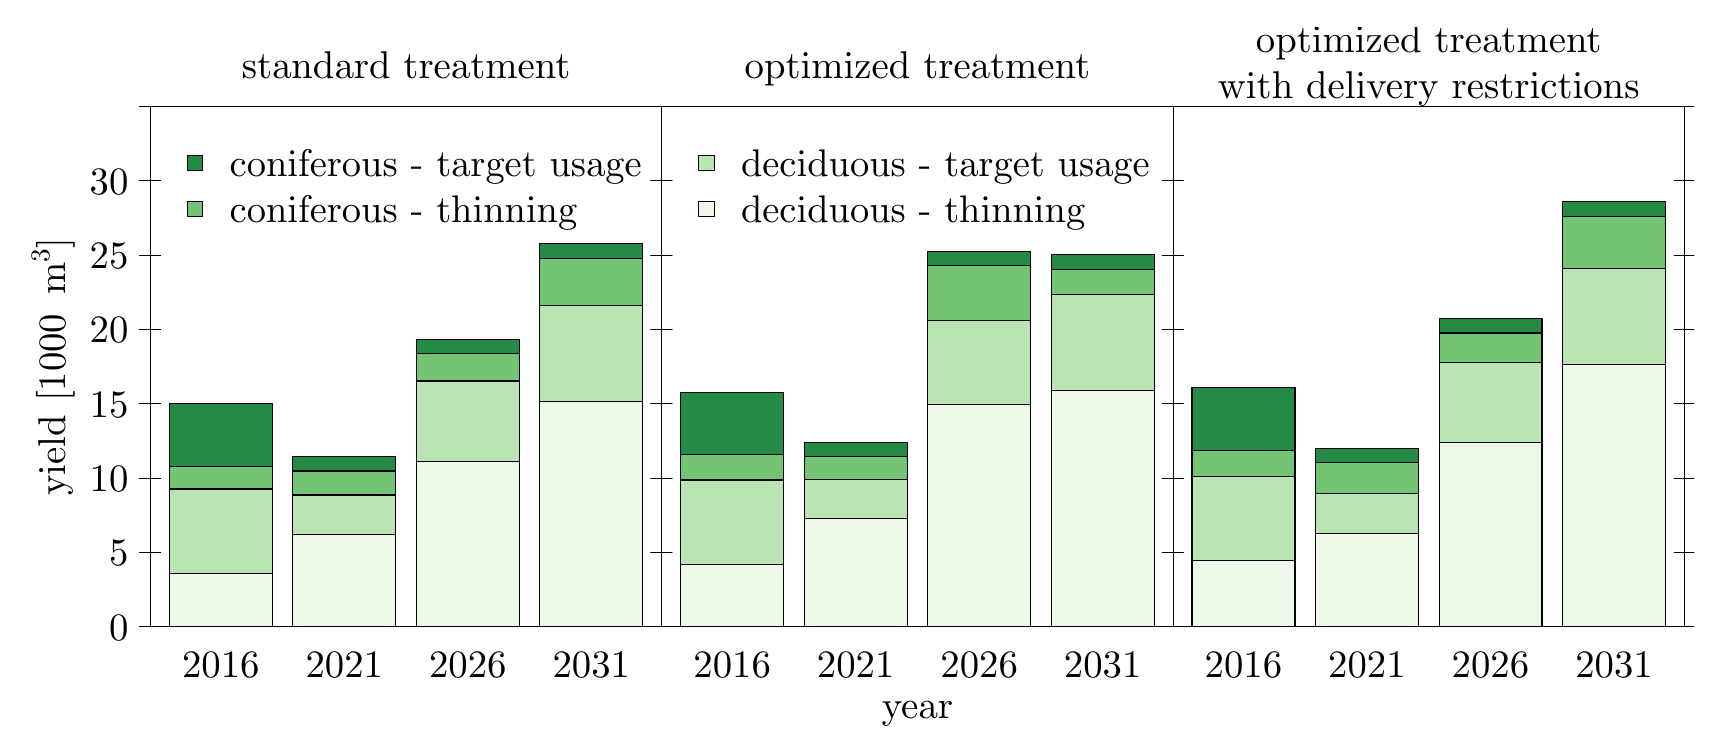
\begin{tikzpicture}[x=1pt,y=1pt]
\definecolor{fillColor}{RGB}{255,255,255}
\path[use as bounding box,fill=fillColor,fill opacity=0.00] (0,0) rectangle (602.23,252.94);
\begin{scope}
\path[clip] ( 44.35, 36.43) rectangle (229.12,224.43);
\definecolor{drawColor}{RGB}{0,0,0}
\definecolor{fillColor}{RGB}{237,248,233}

\path[draw=drawColor,line width= 0.4pt,line join=round,line cap=round,fill=fillColor] ( 51.20, 36.43) rectangle ( 88.39, 55.69);
\definecolor{fillColor}{RGB}{186,228,179}

\path[draw=drawColor,line width= 0.4pt,line join=round,line cap=round,fill=fillColor] ( 51.20, 55.69) rectangle ( 88.39, 86.24);
\definecolor{fillColor}{RGB}{116,196,118}

\path[draw=drawColor,line width= 0.4pt,line join=round,line cap=round,fill=fillColor] ( 51.20, 86.24) rectangle ( 88.39, 94.31);
\definecolor{fillColor}{RGB}{35,139,69}

\path[draw=drawColor,line width= 0.4pt,line join=round,line cap=round,fill=fillColor] ( 51.20, 94.31) rectangle ( 88.39,117.00);
\definecolor{fillColor}{RGB}{237,248,233}

\path[draw=drawColor,line width= 0.4pt,line join=round,line cap=round,fill=fillColor] ( 95.83, 36.43) rectangle (133.02, 69.72);
\definecolor{fillColor}{RGB}{186,228,179}

\path[draw=drawColor,line width= 0.4pt,line join=round,line cap=round,fill=fillColor] ( 95.83, 69.72) rectangle (133.02, 84.07);
\definecolor{fillColor}{RGB}{116,196,118}

\path[draw=drawColor,line width= 0.4pt,line join=round,line cap=round,fill=fillColor] ( 95.83, 84.07) rectangle (133.02, 92.74);
\definecolor{fillColor}{RGB}{35,139,69}

\path[draw=drawColor,line width= 0.4pt,line join=round,line cap=round,fill=fillColor] ( 95.83, 92.74) rectangle (133.02, 98.01);
\definecolor{fillColor}{RGB}{237,248,233}

\path[draw=drawColor,line width= 0.4pt,line join=round,line cap=round,fill=fillColor] (140.46, 36.43) rectangle (177.65, 96.30);
\definecolor{fillColor}{RGB}{186,228,179}

\path[draw=drawColor,line width= 0.4pt,line join=round,line cap=round,fill=fillColor] (140.46, 96.30) rectangle (177.65,125.25);
\definecolor{fillColor}{RGB}{116,196,118}

\path[draw=drawColor,line width= 0.4pt,line join=round,line cap=round,fill=fillColor] (140.46,125.25) rectangle (177.65,135.10);
\definecolor{fillColor}{RGB}{35,139,69}

\path[draw=drawColor,line width= 0.4pt,line join=round,line cap=round,fill=fillColor] (140.46,135.10) rectangle (177.65,140.36);
\definecolor{fillColor}{RGB}{237,248,233}

\path[draw=drawColor,line width= 0.4pt,line join=round,line cap=round,fill=fillColor] (185.09, 36.43) rectangle (222.28,117.84);
\definecolor{fillColor}{RGB}{186,228,179}

\path[draw=drawColor,line width= 0.4pt,line join=round,line cap=round,fill=fillColor] (185.09,117.84) rectangle (222.28,152.47);
\definecolor{fillColor}{RGB}{116,196,118}

\path[draw=drawColor,line width= 0.4pt,line join=round,line cap=round,fill=fillColor] (185.09,152.47) rectangle (222.28,169.50);
\definecolor{fillColor}{RGB}{35,139,69}

\path[draw=drawColor,line width= 0.4pt,line join=round,line cap=round,fill=fillColor] (185.09,169.50) rectangle (222.28,174.87);
\end{scope}
\begin{scope}
\path[clip] (  0.00,  0.00) rectangle (602.23,252.94);
\definecolor{drawColor}{RGB}{0,0,0}

\node[text=drawColor,anchor=base,inner sep=0pt, outer sep=0pt, scale=  1.40] at (136.74,234.45) {standard treatment};

\path[draw=drawColor,line width= 0.4pt,line join=round,line cap=round] ( 44.35, 36.43) -- ( 40.39, 36.43);

\path[draw=drawColor,line width= 0.4pt,line join=round,line cap=round] ( 44.35, 63.29) -- ( 40.39, 63.29);

\path[draw=drawColor,line width= 0.4pt,line join=round,line cap=round] ( 44.35, 90.15) -- ( 40.39, 90.15);

\path[draw=drawColor,line width= 0.4pt,line join=round,line cap=round] ( 44.35,117.00) -- ( 40.39,117.00);

\path[draw=drawColor,line width= 0.4pt,line join=round,line cap=round] ( 44.35,143.86) -- ( 40.39,143.86);

\path[draw=drawColor,line width= 0.4pt,line join=round,line cap=round] ( 44.35,170.72) -- ( 40.39,170.72);

\path[draw=drawColor,line width= 0.4pt,line join=round,line cap=round] ( 44.35,197.58) -- ( 40.39,197.58);

\path[draw=drawColor,line width= 0.4pt,line join=round,line cap=round] ( 44.35,224.43) -- ( 40.39,224.43);

\node[text=drawColor,anchor=base east,inner sep=0pt, outer sep=0pt, scale=  1.40] at ( 36.43, 31.61) {0};

\node[text=drawColor,anchor=base east,inner sep=0pt, outer sep=0pt, scale=  1.40] at ( 36.43, 58.47) {5};

\node[text=drawColor,anchor=base east,inner sep=0pt, outer sep=0pt, scale=  1.40] at ( 36.43, 85.33) {10};

\node[text=drawColor,anchor=base east,inner sep=0pt, outer sep=0pt, scale=  1.40] at ( 36.43,112.18) {15};

\node[text=drawColor,anchor=base east,inner sep=0pt, outer sep=0pt, scale=  1.40] at ( 36.43,139.04) {20};

\node[text=drawColor,anchor=base east,inner sep=0pt, outer sep=0pt, scale=  1.40] at ( 36.43,165.90) {25};

\node[text=drawColor,anchor=base east,inner sep=0pt, outer sep=0pt, scale=  1.40] at ( 36.43,192.75) {30};

\path[draw=drawColor,line width= 0.4pt,line join=round,line cap=round] ( 44.35, 36.43) -- ( 48.05, 36.43);

\path[draw=drawColor,line width= 0.4pt,line join=round,line cap=round] ( 44.35, 63.29) -- ( 48.05, 63.29);

\path[draw=drawColor,line width= 0.4pt,line join=round,line cap=round] ( 44.35, 90.15) -- ( 48.05, 90.15);

\path[draw=drawColor,line width= 0.4pt,line join=round,line cap=round] ( 44.35,117.00) -- ( 48.05,117.00);

\path[draw=drawColor,line width= 0.4pt,line join=round,line cap=round] ( 44.35,143.86) -- ( 48.05,143.86);

\path[draw=drawColor,line width= 0.4pt,line join=round,line cap=round] ( 44.35,170.72) -- ( 48.05,170.72);

\path[draw=drawColor,line width= 0.4pt,line join=round,line cap=round] ( 44.35,197.58) -- ( 48.05,197.58);

\node[text=drawColor,anchor=base,inner sep=0pt, outer sep=0pt, scale=  1.40] at ( 69.79, 18.22) {2016};

\node[text=drawColor,anchor=base,inner sep=0pt, outer sep=0pt, scale=  1.40] at (114.42, 18.22) {2021};

\node[text=drawColor,anchor=base,inner sep=0pt, outer sep=0pt, scale=  1.40] at (159.05, 18.22) {2026};

\node[text=drawColor,anchor=base,inner sep=0pt, outer sep=0pt, scale=  1.40] at (203.68, 18.22) {2031};

\node[text=drawColor,rotate= 90.00,anchor=base west,inner sep=0pt, outer sep=0pt, scale=  1.40] at ( 13.53, 83.86) {yield [1000};

\node[text=drawColor,rotate= 90.00,anchor=base west,inner sep=0pt, outer sep=0pt, scale=  1.40] at ( 13.53,149.56) { };

\node[text=drawColor,rotate= 90.00,anchor=base west,inner sep=0pt, outer sep=0pt, scale=  1.40] at ( 13.53,156.56) {m};

\node[text=drawColor,rotate= 90.00,anchor=base west,inner sep=0pt, outer sep=0pt, scale=  0.98] at (  7.80,168.22) {3};

\node[text=drawColor,rotate= 90.00,anchor=base west,inner sep=0pt, outer sep=0pt, scale=  1.40] at ( 13.53,173.12) {]};
\end{scope}
\begin{scope}
\path[clip] ( 44.35, 36.43) rectangle (229.12,224.43);
\definecolor{drawColor}{RGB}{0,0,0}
\definecolor{fillColor}{RGB}{35,139,69}

\path[draw=drawColor,line width= 0.4pt,line join=round,line cap=round,fill=fillColor] ( 57.76,201.28) rectangle ( 63.29,206.80);
\definecolor{fillColor}{RGB}{116,196,118}

\path[draw=drawColor,line width= 0.4pt,line join=round,line cap=round,fill=fillColor] ( 57.76,184.65) rectangle ( 63.29,190.17);

\node[text=drawColor,anchor=base west,inner sep=0pt, outer sep=0pt, scale=  1.39] at ( 73.00,199.27) {coniferous - target usage};

\node[text=drawColor,anchor=base west,inner sep=0pt, outer sep=0pt, scale=  1.39] at ( 73.00,182.64) {coniferous - thinning};
\end{scope}
\begin{scope}
\path[clip] (  0.00,  0.00) rectangle (602.23,252.94);
\definecolor{drawColor}{RGB}{0,0,0}

\path[draw=drawColor,line width= 0.4pt,line join=round,line cap=round] ( 44.35, 36.43) --
	(229.12, 36.43) --
	(229.12,224.43) --
	( 44.35,224.43) --
	( 44.35, 36.43);
\end{scope}
\begin{scope}
\path[clip] (229.12, 36.43) rectangle (413.89,224.43);
\definecolor{drawColor}{RGB}{0,0,0}
\definecolor{fillColor}{RGB}{237,248,233}

\path[draw=drawColor,line width= 0.4pt,line join=round,line cap=round,fill=fillColor] (235.97, 36.43) rectangle (273.16, 58.94);
\definecolor{fillColor}{RGB}{186,228,179}

\path[draw=drawColor,line width= 0.4pt,line join=round,line cap=round,fill=fillColor] (235.97, 58.94) rectangle (273.16, 89.49);
\definecolor{fillColor}{RGB}{116,196,118}

\path[draw=drawColor,line width= 0.4pt,line join=round,line cap=round,fill=fillColor] (235.97, 89.49) rectangle (273.16, 98.56);
\definecolor{fillColor}{RGB}{35,139,69}

\path[draw=drawColor,line width= 0.4pt,line join=round,line cap=round,fill=fillColor] (235.97, 98.56) rectangle (273.16,121.25);
\definecolor{fillColor}{RGB}{237,248,233}

\path[draw=drawColor,line width= 0.4pt,line join=round,line cap=round,fill=fillColor] (280.60, 36.43) rectangle (317.79, 75.43);
\definecolor{fillColor}{RGB}{186,228,179}

\path[draw=drawColor,line width= 0.4pt,line join=round,line cap=round,fill=fillColor] (280.60, 75.43) rectangle (317.79, 89.78);
\definecolor{fillColor}{RGB}{116,196,118}

\path[draw=drawColor,line width= 0.4pt,line join=round,line cap=round,fill=fillColor] (280.60, 89.78) rectangle (317.79, 97.89);
\definecolor{fillColor}{RGB}{35,139,69}

\path[draw=drawColor,line width= 0.4pt,line join=round,line cap=round,fill=fillColor] (280.60, 97.89) rectangle (317.79,103.16);
\definecolor{fillColor}{RGB}{237,248,233}

\path[draw=drawColor,line width= 0.4pt,line join=round,line cap=round,fill=fillColor] (325.23, 36.43) rectangle (362.42,116.66);
\definecolor{fillColor}{RGB}{186,228,179}

\path[draw=drawColor,line width= 0.4pt,line join=round,line cap=round,fill=fillColor] (325.23,116.66) rectangle (362.42,147.07);
\definecolor{fillColor}{RGB}{116,196,118}

\path[draw=drawColor,line width= 0.4pt,line join=round,line cap=round,fill=fillColor] (325.23,147.07) rectangle (362.42,166.93);
\definecolor{fillColor}{RGB}{35,139,69}

\path[draw=drawColor,line width= 0.4pt,line join=round,line cap=round,fill=fillColor] (325.23,166.93) rectangle (362.42,172.20);
\definecolor{fillColor}{RGB}{237,248,233}

\path[draw=drawColor,line width= 0.4pt,line join=round,line cap=round,fill=fillColor] (369.86, 36.43) rectangle (407.05,121.75);
\definecolor{fillColor}{RGB}{186,228,179}

\path[draw=drawColor,line width= 0.4pt,line join=round,line cap=round,fill=fillColor] (369.86,121.75) rectangle (407.05,156.43);
\definecolor{fillColor}{RGB}{116,196,118}

\path[draw=drawColor,line width= 0.4pt,line join=round,line cap=round,fill=fillColor] (369.86,156.43) rectangle (407.05,165.56);
\definecolor{fillColor}{RGB}{35,139,69}

\path[draw=drawColor,line width= 0.4pt,line join=round,line cap=round,fill=fillColor] (369.86,165.56) rectangle (407.05,170.92);
\end{scope}
\begin{scope}
\path[clip] (  0.00,  0.00) rectangle (602.23,252.94);
\definecolor{drawColor}{RGB}{0,0,0}

\path[draw=drawColor,line width= 0.4pt,line join=round,line cap=round] (229.12, 36.43) -- (225.16, 36.43);

\path[draw=drawColor,line width= 0.4pt,line join=round,line cap=round] (229.12, 63.29) -- (225.16, 63.29);

\path[draw=drawColor,line width= 0.4pt,line join=round,line cap=round] (229.12, 90.15) -- (225.16, 90.15);

\path[draw=drawColor,line width= 0.4pt,line join=round,line cap=round] (229.12,117.00) -- (225.16,117.00);

\path[draw=drawColor,line width= 0.4pt,line join=round,line cap=round] (229.12,143.86) -- (225.16,143.86);

\path[draw=drawColor,line width= 0.4pt,line join=round,line cap=round] (229.12,170.72) -- (225.16,170.72);

\path[draw=drawColor,line width= 0.4pt,line join=round,line cap=round] (229.12,197.58) -- (225.16,197.58);

\path[draw=drawColor,line width= 0.4pt,line join=round,line cap=round] (229.12, 36.43) -- (232.82, 36.43);

\path[draw=drawColor,line width= 0.4pt,line join=round,line cap=round] (229.12, 63.29) -- (232.82, 63.29);

\path[draw=drawColor,line width= 0.4pt,line join=round,line cap=round] (229.12, 90.15) -- (232.82, 90.15);

\path[draw=drawColor,line width= 0.4pt,line join=round,line cap=round] (229.12,117.00) -- (232.82,117.00);

\path[draw=drawColor,line width= 0.4pt,line join=round,line cap=round] (229.12,143.86) -- (232.82,143.86);

\path[draw=drawColor,line width= 0.4pt,line join=round,line cap=round] (229.12,170.72) -- (232.82,170.72);

\path[draw=drawColor,line width= 0.4pt,line join=round,line cap=round] (229.12,197.58) -- (232.82,197.58);

\node[text=drawColor,anchor=base,inner sep=0pt, outer sep=0pt, scale=  1.40] at (254.56, 18.22) {2016};

\node[text=drawColor,anchor=base,inner sep=0pt, outer sep=0pt, scale=  1.40] at (299.19, 18.22) {2021};

\node[text=drawColor,anchor=base,inner sep=0pt, outer sep=0pt, scale=  1.40] at (343.82, 18.22) {2026};

\node[text=drawColor,anchor=base,inner sep=0pt, outer sep=0pt, scale=  1.40] at (388.45, 18.22) {2031};

\path[draw=drawColor,line width= 0.4pt,line join=round,line cap=round] (229.12, 36.43) --
	(413.89, 36.43) --
	(413.89,224.43) --
	(229.12,224.43) --
	(229.12, 36.43);
\end{scope}
\begin{scope}
\path[clip] (229.12, 36.43) rectangle (413.89,224.43);
\definecolor{drawColor}{RGB}{0,0,0}
\definecolor{fillColor}{RGB}{186,228,179}

\path[draw=drawColor,line width= 0.4pt,line join=round,line cap=round,fill=fillColor] (242.53,201.28) rectangle (248.06,206.80);
\definecolor{fillColor}{RGB}{237,248,233}

\path[draw=drawColor,line width= 0.4pt,line join=round,line cap=round,fill=fillColor] (242.53,184.65) rectangle (248.06,190.17);

\node[text=drawColor,anchor=base west,inner sep=0pt, outer sep=0pt, scale=  1.39] at (257.77,199.27) {deciduous - target usage};

\node[text=drawColor,anchor=base west,inner sep=0pt, outer sep=0pt, scale=  1.39] at (257.77,182.64) {deciduous - thinning};
\end{scope}
\begin{scope}
\path[clip] (  0.00,  0.00) rectangle (602.23,252.94);
\definecolor{drawColor}{RGB}{0,0,0}

\node[text=drawColor,anchor=base,inner sep=0pt, outer sep=0pt, scale=  1.40] at (321.51,234.45) {optimized treatment};

\node[text=drawColor,anchor=base,inner sep=0pt, outer sep=0pt, scale=  1.40] at (321.51,  3.17) {year};
\end{scope}
\begin{scope}
\path[clip] (413.89, 36.43) rectangle (598.66,224.43);
\definecolor{drawColor}{RGB}{0,0,0}
\definecolor{fillColor}{RGB}{237,248,233}

\path[draw=drawColor,line width= 0.4pt,line join=round,line cap=round,fill=fillColor] (420.74, 36.43) rectangle (457.93, 60.28);
\definecolor{fillColor}{RGB}{186,228,179}

\path[draw=drawColor,line width= 0.4pt,line join=round,line cap=round,fill=fillColor] (420.74, 60.28) rectangle (457.93, 90.83);
\definecolor{fillColor}{RGB}{116,196,118}

\path[draw=drawColor,line width= 0.4pt,line join=round,line cap=round,fill=fillColor] (420.74, 90.83) rectangle (457.93,100.30);
\definecolor{fillColor}{RGB}{35,139,69}

\path[draw=drawColor,line width= 0.4pt,line join=round,line cap=round,fill=fillColor] (420.74,100.30) rectangle (457.93,122.99);
\definecolor{fillColor}{RGB}{237,248,233}

\path[draw=drawColor,line width= 0.4pt,line join=round,line cap=round,fill=fillColor] (465.37, 36.43) rectangle (502.56, 70.21);
\definecolor{fillColor}{RGB}{186,228,179}

\path[draw=drawColor,line width= 0.4pt,line join=round,line cap=round,fill=fillColor] (465.37, 70.21) rectangle (502.56, 84.56);
\definecolor{fillColor}{RGB}{116,196,118}

\path[draw=drawColor,line width= 0.4pt,line join=round,line cap=round,fill=fillColor] (465.37, 84.56) rectangle (502.56, 95.89);
\definecolor{fillColor}{RGB}{35,139,69}

\path[draw=drawColor,line width= 0.4pt,line join=round,line cap=round,fill=fillColor] (465.37, 95.89) rectangle (502.56,100.79);
\definecolor{fillColor}{RGB}{237,248,233}

\path[draw=drawColor,line width= 0.4pt,line join=round,line cap=round,fill=fillColor] (510.00, 36.43) rectangle (547.19,102.92);
\definecolor{fillColor}{RGB}{186,228,179}

\path[draw=drawColor,line width= 0.4pt,line join=round,line cap=round,fill=fillColor] (510.00,102.92) rectangle (547.19,131.87);
\definecolor{fillColor}{RGB}{116,196,118}

\path[draw=drawColor,line width= 0.4pt,line join=round,line cap=round,fill=fillColor] (510.00,131.87) rectangle (547.19,142.60);
\definecolor{fillColor}{RGB}{35,139,69}

\path[draw=drawColor,line width= 0.4pt,line join=round,line cap=round,fill=fillColor] (510.00,142.60) rectangle (547.19,147.86);
\definecolor{fillColor}{RGB}{237,248,233}

\path[draw=drawColor,line width= 0.4pt,line join=round,line cap=round,fill=fillColor] (554.63, 36.43) rectangle (591.82,131.15);
\definecolor{fillColor}{RGB}{186,228,179}

\path[draw=drawColor,line width= 0.4pt,line join=round,line cap=round,fill=fillColor] (554.63,131.15) rectangle (591.82,165.80);
\definecolor{fillColor}{RGB}{116,196,118}

\path[draw=drawColor,line width= 0.4pt,line join=round,line cap=round,fill=fillColor] (554.63,165.80) rectangle (591.82,184.80);
\definecolor{fillColor}{RGB}{35,139,69}

\path[draw=drawColor,line width= 0.4pt,line join=round,line cap=round,fill=fillColor] (554.63,184.80) rectangle (591.82,190.16);
\end{scope}
\begin{scope}
\path[clip] (  0.00,  0.00) rectangle (602.23,252.94);
\definecolor{drawColor}{RGB}{0,0,0}

\path[draw=drawColor,line width= 0.4pt,line join=round,line cap=round] (413.89, 36.43) -- (409.93, 36.43);

\path[draw=drawColor,line width= 0.4pt,line join=round,line cap=round] (413.89, 63.29) -- (409.93, 63.29);

\path[draw=drawColor,line width= 0.4pt,line join=round,line cap=round] (413.89, 90.15) -- (409.93, 90.15);

\path[draw=drawColor,line width= 0.4pt,line join=round,line cap=round] (413.89,117.00) -- (409.93,117.00);

\path[draw=drawColor,line width= 0.4pt,line join=round,line cap=round] (413.89,143.86) -- (409.93,143.86);

\path[draw=drawColor,line width= 0.4pt,line join=round,line cap=round] (413.89,170.72) -- (409.93,170.72);

\path[draw=drawColor,line width= 0.4pt,line join=round,line cap=round] (413.89,197.58) -- (409.93,197.58);

\path[draw=drawColor,line width= 0.4pt,line join=round,line cap=round] (413.89, 36.43) -- (417.59, 36.43);

\path[draw=drawColor,line width= 0.4pt,line join=round,line cap=round] (413.89, 63.29) -- (417.59, 63.29);

\path[draw=drawColor,line width= 0.4pt,line join=round,line cap=round] (413.89, 90.15) -- (417.59, 90.15);

\path[draw=drawColor,line width= 0.4pt,line join=round,line cap=round] (413.89,117.00) -- (417.59,117.00);

\path[draw=drawColor,line width= 0.4pt,line join=round,line cap=round] (413.89,143.86) -- (417.59,143.86);

\path[draw=drawColor,line width= 0.4pt,line join=round,line cap=round] (413.89,170.72) -- (417.59,170.72);

\path[draw=drawColor,line width= 0.4pt,line join=round,line cap=round] (413.89,197.58) -- (417.59,197.58);

\path[draw=drawColor,line width= 0.4pt,line join=round,line cap=round] (598.66, 36.43) -- (602.23, 36.43);

\path[draw=drawColor,line width= 0.4pt,line join=round,line cap=round] (598.66, 63.29) -- (602.23, 63.29);

\path[draw=drawColor,line width= 0.4pt,line join=round,line cap=round] (598.66, 90.15) -- (602.23, 90.15);

\path[draw=drawColor,line width= 0.4pt,line join=round,line cap=round] (598.66,117.00) -- (602.23,117.00);

\path[draw=drawColor,line width= 0.4pt,line join=round,line cap=round] (598.66,143.86) -- (602.23,143.86);

\path[draw=drawColor,line width= 0.4pt,line join=round,line cap=round] (598.66,170.72) -- (602.23,170.72);

\path[draw=drawColor,line width= 0.4pt,line join=round,line cap=round] (598.66,197.58) -- (602.23,197.58);

\path[draw=drawColor,line width= 0.4pt,line join=round,line cap=round] (598.66,224.43) -- (602.23,224.43);

\path[draw=drawColor,line width= 0.4pt,line join=round,line cap=round] (598.66, 36.43) -- (594.97, 36.43);

\path[draw=drawColor,line width= 0.4pt,line join=round,line cap=round] (598.66, 63.29) -- (594.97, 63.29);

\path[draw=drawColor,line width= 0.4pt,line join=round,line cap=round] (598.66, 90.15) -- (594.97, 90.15);

\path[draw=drawColor,line width= 0.4pt,line join=round,line cap=round] (598.66,117.00) -- (594.97,117.00);

\path[draw=drawColor,line width= 0.4pt,line join=round,line cap=round] (598.66,143.86) -- (594.97,143.86);

\path[draw=drawColor,line width= 0.4pt,line join=round,line cap=round] (598.66,170.72) -- (594.97,170.72);

\path[draw=drawColor,line width= 0.4pt,line join=round,line cap=round] (598.66,197.58) -- (594.97,197.58);

\node[text=drawColor,anchor=base,inner sep=0pt, outer sep=0pt, scale=  1.40] at (439.33, 18.22) {2016};

\node[text=drawColor,anchor=base,inner sep=0pt, outer sep=0pt, scale=  1.40] at (483.96, 18.22) {2021};

\node[text=drawColor,anchor=base,inner sep=0pt, outer sep=0pt, scale=  1.40] at (528.59, 18.22) {2026};

\node[text=drawColor,anchor=base,inner sep=0pt, outer sep=0pt, scale=  1.40] at (573.22, 18.22) {2031};

\node[text=drawColor,anchor=base,inner sep=0pt, outer sep=0pt, scale=  1.40] at (506.28,244.09) {optimized treatment};

\node[text=drawColor,anchor=base,inner sep=0pt, outer sep=0pt, scale=  1.40] at (506.28,227.29) {with delivery restrictions};

\path[draw=drawColor,line width= 0.4pt,line join=round,line cap=round] (413.89, 36.43) --
	(598.66, 36.43) --
	(598.66,224.43) --
	(413.89,224.43) --
	(413.89, 36.43);
\end{scope}
\end{tikzpicture}
